%%%%%%%%%%%%%%%%%%%%%%%%%%%%%%%%%%%%%%%%%%%%%%%%%%%%%%%%%%%%
%%  This Beamer template was created by Cameron Bracken.
%%  Anyone can freely use or modify it for any purpose
%%  without attribution.
%%
%%  Last Modified: January 9, 2009
%%

\documentclass[xcolor=x11names,compress]{beamer}

%% General document %%%%%%%%%%%%%%%%%%%%%%%%%%%%%%%%%%
\usepackage{booktabs}
\usepackage{graphicx}
\usepackage[spanish]{babel}
\usepackage[utf8]{inputenc}
\usepackage{tikz}
\usetikzlibrary{decorations.fractals}
%%%%%%%%%%%%%%%%%%%%%%%%%%%%%%%%%%%%%%%%%%%%%%%%%%%%%%


%% Beamer Layout %%%%%%%%%%%%%%%%%%%%%%%%%%%%%%%%%%
\useoutertheme[subsection=false,shadow]{miniframes}
\useinnertheme{default}
\usefonttheme{serif}
\usepackage{palatino}

\setbeamerfont{title like}{shape=\scshape}
\setbeamerfont{frametitle}{shape=\scshape}

\setbeamercolor*{lower separation line head}{bg=DeepSkyBlue4} 
\setbeamercolor*{normal text}{fg=black,bg=white} 
\setbeamercolor*{alerted text}{fg=red} 
\setbeamercolor*{example text}{fg=blue} 
\setbeamercolor*{structure}{fg=black} 
 
\setbeamercolor*{palette tertiary}{fg=black,bg=black!10} 
\setbeamercolor*{palette quaternary}{fg=black,bg=black!10} 

\renewcommand{\(}{\begin{columns}}
\renewcommand{\)}{\end{columns}}
\newcommand{\<}[1]{\begin{column}{#1}}
\renewcommand{\>}{\end{column}}
%%%%%%%%%%%%%%%%%%%%%%%%%%%%%%%%%%%%%%%%%%%%%%%%%%




\begin{document}


%%%%%%%%%%%%%%%%%%%%%%%%%%%%%%%%%%%%%%%%%%%%%%%%%%%%%%
%%%%%%%%%%%%%%%%%%%%%%%%%%%%%%%%%%%%%%%%%%%%%%%%%%%%%%
%\section{\scshape Introduction}
\begin{frame}
\title{Modelo de mezclas Gaussianas (GMM)}
%\subtitle{SUBTITLE}
\author{
	{\scriptsize Rafael Pérez Torres\\\vspace{1cm}
	Tópicos Selectos en Reconocimiento de Patrones\\
	Profesor: Dr. Wilfrido Gómez Flores\\
	}{\it LTI Cinvestav}\\
}
\date{
	\begin{tikzpicture}[decoration=Koch curve type 2] 
		\draw[DeepSkyBlue4] decorate{ decorate{ decorate{ (0,0) -- (3,0) }}}; 
	\end{tikzpicture}  
	\\
	\vspace{1cm}
	29 de mayo 2015
}
\titlepage
\end{frame}

%%%%%%%%%%%%%%%%%%%%%%%%%%%%%%%%%%%%%%%%%%%%%%%%%%%%%%
%%%%%%%%%%%%%%%%%%%%%%%%%%%%%%%%%%%%%%%%%%%%%%%%%%%%%%
\begin{frame}{Agenda}
\tableofcontents
\end{frame}

%%%%%%%%%%%%%%%%%%%%%%%%%%%%%%%%%%%%%%%%%%%%%%%%%%%%%%
%%%%%%%%%%%%%%%%%%%%%%%%%%%%%%%%%%%%%%%%%%%%%%%%%%%%%%
\section{\scshape Introducción}
\subsection{Introducción}
\begin{frame}{Introducción}
\begin{itemize}
	\item Normalmente, la naturaleza de una distribución refleja características intrínsecas en los datos.
	\item Las técnicas de agrupamiento basadas en distribución intentan crear un modelo parametrizado que describa a los datos.
	\item Con el modelo es posible realizar inferencias que sean útiles para labores de identificación - agrupamiento
\end{itemize}
\end{frame}

\begin{frame}{Introducción}
\begin{itemize}
 	\item El modelo que describe a una distribución puede ser conocido a través de una \emph{PDF} (Probability Density Function).
 	\item Normalmente, los datos que provienen del mundo real obedecen a una distribución normal o gaussiana, definida como
\begin{equation}
 g(x|\mu _i,\Sigma_i)  = \frac{1}{(2 \pi)^{(l/2)}}\text{exp} \left(  -\frac{1}{2}(x-\mu _i)^T \Sigma _i^{-1} (x-\mu _i) \right)
\end{equation}
 Esta PDF es parametrizada por las medias $\mu$ y covarianzas $\Sigma$ de los datos.
\end{itemize}    
\end{frame}


\begin{frame}{Introducción}
\begin{itemize}
	\item En general, las técnicas de agrupamiento asumen que los datos han sido generados por una mezcla de distribuciones (PDF).
	\item Cada componente de la mezcla define a cada uno de los grupos.
\end{itemize}
\end{frame}
%%%%%%%%%%%%%%%%%%%%%%%%%%%%%%%%%%%%%%%%%%%%%%%%%%%%%%
%%%%%%%%%%%%%%%%%%%%%%%%%%%%%%%%%%%%%%%%%%%%%%%%%%%%%%

\section{\scshape GMM}
\subsection{El modelo de mezclas Gaussianas (GMM)}
\begin{frame}{El modelo de mezclas Gaussianas (GMM)}
   
   	\begin{itemize}
   		\item El GMM es una suma ponderada de $M$ PDFs Gaussianas, expresado como
   		\begin{equation}
p(x|\omega _i,\Sigma _i) = \sum_{i=1}^{M}\omega _ig(x|\mu _i,\Sigma_i)
\end{equation}
Donde $g(x|\mu _i,\Sigma_i)$ es la PDF gaussiana de cada grupo y $\omega _i$ es el vector de coeficientes mixtos que se encuentra sujeto a la restricción $\sum_{i=1}^{M}\omega _i = 1$.
   	\end{itemize}

\begin{figure}
	\centering
	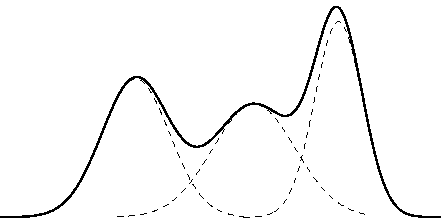
\includegraphics[scale=0.3]{../resources/images/gmm}
	\caption{Una combinación de PDFs Gaussianas}
	\label{fig:figure1}
\end{figure}
\end{frame}

\begin{frame}{El modelo de mezclas Gaussianas (GMM)}
\begin{itemize}
	\item Entonces, el GMM es parametrizado por los vectores de medias, covarianzas y coeficientes de cada grupo:
		$$
		\lambda = \{ \omega _i, \mu _i, \Sigma _i \}
		$$
		\item El resto del trabajo consiste en encontrar los valores adecuados para dichos parámetros.
\end{itemize}  
\end{frame}

%%%%%%%%%%%%%%%%%%%%%%%%%%%%%%%%%%%%%%%%%%%%%%%%%%%%%%
%%%%%%%%%%%%%%%%%%%%%%%%%%%%%%%%%%%%%%%%%%%%%%%%%%%%%%
\section{\scshape Parámetros del GMM}
\subsection{Estimación de los parámetros GMM}
\begin{frame}{Estimación de los parámetros del GMM}
   	\begin{itemize}
   		\item Existen varios métoos para estimar $\lambda$ de un GMM.
   		\item El más utilizado es el método de estimación de máxima verosimilitud (ML).
   		\item El objetivo del método de ML es maximizar la verosimilitud del GMM dado el conjunto de datos de entrenamiento.
   	\end{itemize}
\end{frame}

\subsection{Descripción del método de máxima verosimilitud}
\begin{frame}{El método de máxima verosimilitud}   	
Sea $\mathcal{X}$ una variable aleatoria con función de probabilidad $p(\mathcal{X};\theta)$ donde $\theta$ es un parámetro desconocido.

Además, sean $x_1,x_2,\ldots ,x_N$ los valores observados en una muestra aleatoria de tamaño $N$ de la misma variable.

La función de verosimilitud de la muestra (o función de densidad conjunta) es:
\begin{equation}
\mathcal{L}(\theta) = p(\mathcal{X};\theta) = p(x_1,x_2,\ldots,x_n ; \theta) = \prod_{i=1}^N p(x_i ; \theta)
\end{equation}
\end{frame}

\begin{frame}{El método de máxima verosimilitud, ejemplo}
\begin{itemize}
	\item Se desea estimar la probabilidad $p$ de que salga cara en el lanzamiento de una moneda (no necesariamente regular).
	\item Se lanza cinco veces la moneda y se obtiene: $C+CC+$
	\item $p(C+CC+) = p * (1 - p) * p * p * (1 - p) = p^3 (1 - p)^2$
\end{itemize}
\begin{table}[h]
\tiny
\centering
\begin{tabular}{@{}cc@{}}
\toprule
\textbf{Valor de $p$} & \textbf{Probabilidad de la muestra observada} \\ \midrule
0.0                 & 0.0000                                        \\
0.1                 & 0.0008                                        \\
0.2                 & 0.0051                                        \\
0.3                 & 0.0132                                        \\
0.4                 & 0.0230                                        \\
0.5                 & 0.0313                                        \\
0.6                 & 0.0346                                        \\
0.7                 & 0.0309                                        \\
0.8                 & 0.0205                                         \\
0.9                 & 0.0073                                        \\
1.0                 & 0.0000                                        \\ \bottomrule
\end{tabular}
\caption{Valores obtenidos para distintos valores de $p$}
\end{table}
\end{frame}

\begin{frame}{El método de máxima verosimilitud, ejemplo}
\begin{equation}
p(k \text{ caras en} n \text{ lanzamientos}) = {n \choose k} p^k (1 - p)^{n-k} = \mathcal{L}(p)
\end{equation}

Derivando e igualando a 0
\begin{equation}
\frac{\partial \text{ ln}\big ( \mathcal{L}(p)  \big )}{\partial p} = \frac{k}{p} - \frac{n-k}{1-p}
\label{eq:pasos-frec-2}
\end{equation}

\begin{eqnarray}
\frac{k}{\hat{p}} - \frac{n-k}{1-\hat{p}} = 0 \to k(1-\hat{p}) - \hat{p}(n-k) = 0 \label{eq:pasos-frec-3} \to \hat{p} = \frac{k}{n}
\label{eq:pasos-frec-4}
\end{eqnarray}
 El \emph{estimador máximo verosimil} de la probabilidad de un suceso es la frecuencia relativa.
\end{frame}

\begin{frame}{ML en distribuciones normales}
Al aplicar ML a distribuciones Gaussianas, se observa que los estimadores máximos verosímiles coinciden con la $\mu$ y la $\Sigma$.

\begin{eqnarray}
\mathcal{L}(\mu,\sigma ^2) &=& \text{ln}\prod_{i=1}^N p(x_i;\theta) \label{eq:pasos-1} \\ &=& \text{ ln}\prod_{i=1}^N \frac{1}{\sqrt{2 \pi}\sqrt{\sigma ^2}} \text{exp} \left ( -\frac{(x_i - \mu)^2}{2 \sigma ^2}  \right ) \label{eq:pasos-2} \\ &=&
-\frac{N}{2} \text{ ln}(2\pi \sigma ^2) - \frac{1}{2 \sigma ^2} \sum_{i=1}^{N}(x - \mu)^2 \label{eq:pasos-3}
\end{eqnarray}

\begin{equation}
\hat{\mu} = \frac{1}{N}\sum_{i=1}^{N}x_i \hspace{1cm} \hat{\sigma}^2 = \frac{1}{N}\sum_{i=1}^{N}(x_i - \hat{\mu})^2
\label{eq:media}
\end{equation}

\end{frame}

%%%%%%%%%%%%%%%%%%%%%%%%%%%%%%%%%%%%%%%%%%%%%%%%%%%%%%
%%%%%%%%%%%%%%%%%%%%%%%%%%%%%%%%%%%%%%%%%%%%%%%%%%%%%%
\section{\scshape El algoritmo EM}
\subsection{Descripción del algoritmo EM}
\begin{frame}{El algoritmo EM}
\begin{itemize}
	\item El algoritmo Expectation-Maximization se basa en el método de estimación de máxima verosimilitud para determinar los valores \emph{óptimos} de los parámetros ($\lambda$) de un GMM.
	\item Se deben calcular las derivadas de los parámetros de la función de log-verosimilitud $\big(\lambda = \{ \mu_k, \Sigma_k, \omega_k \} \big )$:
$$
\text{ln}p(x|\lambda) = \sum_{i=1}^N\text{ln} \left\{ \sum_{k=1}^{M} \omega _k g \left ( x_i | \mu_k,\Sigma_k \right )  \right\}
$$
\end{itemize}
\end{frame}

\begin{frame}{El algoritmo EM} 
\begin{exampleblock}{Pasos del algoritmo EM}
\begin{enumerate}
	\item Selección de valores iniciales para $\lambda$.
	\item Paso E: Evaluar probabilidades a posteriori utilizando el actual conjunto de valores $\lambda$.
	\item Paso M: Reestimar $\lambda$ utilizando las probabilidades a posteriori obtenidas.
	\item Criterio de parada atendiendo a los resultados de la función de verosimilitud de la iteración $t$ y $t-1$.
\end{enumerate}
\end{exampleblock}
\end{frame}

\begin{frame}{EM: Paso 1}
\begin{exampleblock}{Paso 1: Selección de valores iniciales}
\begin{itemize}
	\item El algoritmo EM requiere la cantidad de $M$ componentes Gaussianas a considerar en el GMM y el valor inicial de $\lambda$
	\item Normalmente, se utiliza k-means para obtener el valor de las medias iniciales.
	\item $\Sigma_k$ se calcula en base a todos las instancias pertenecientes al grupo $k$.
	\item Los coeficientes se calculan como $\omega_k = N_k / N$ donde $N_k$ es la cantidad de \emph{instancias} del grupo y $N$ es la cantidad total de instancias.
\end{itemize}
\end{exampleblock}
\end{frame}

\begin{frame}{EM: Paso 2, E}
\begin{exampleblock}{Paso 2: Expectation}
Para la $i$-ésima muestra se calculan las probabilidades a posteriori para la $k$-ésima componente, o en otras palabras, se calcula la probabilidad de que cada muestra pertenezca a cada clúster, mediante:

\begin{equation}
p(k|x_i,\lambda) = \frac{w_k g(x_i | \mu_k,\Sigma_k)}{\sum_{k=1}^{M} w_k g(x_i|\mu_k,\Sigma_k)}
\end{equation}

donde $g(x|\mu _i,\Sigma_i)  = \frac{1}{(2 \pi)^{(l/2)}}\text{exp} \left(  -\frac{1}{2}(x-\mu _i)^T \Sigma _i^{-1} (x-\mu _i) \right)$.

Este paso puede ser considerado similar al paso de asignación de clúster en el algoritmo k-means.
\end{exampleblock}
\end{frame}

\begin{frame}{EM: Paso 3, M}
\begin{exampleblock}{Paso 3: Maximization}
Se reestiman los valores del parámetro $\lambda$, es decir, $\mu_k, \Sigma_k, \omega_k$, a través de:
\begin{equation}
	\hat{\omega _k}^{t+1} = \frac{1}{N} \sum_{i=1}^{N} p(k|x_i,\lambda)
\end{equation}

\begin{equation}
	\hat{\mu _k}^{t+1} = \frac{\sum_{i=1}^{N} p(k|x_i,\lambda) x_i}{\sum_{i=1}^{N} p(k|x_i,\lambda)}
\end{equation}

\begin{equation}
	\hat{\Sigma _k}^{t+1} = \frac{\sum_{i=1}^{N} p\left(  k|x_i,\lambda \right ) \left( x_i - \hat{\mu}_k^{t+1} \right ) \left( x_i - \hat{\mu}_k^{t+1} \right )^T}{\sum_{i=1}^{N} p\left(  k|x_i,\lambda \right )}
\end{equation}

Este paso puede ser considerado similar al paso de recálculo de clústers en el algoritmo k-means.
\end{exampleblock}
\end{frame}

\begin{frame}{EM: Paso 4}
\begin{exampleblock}{Paso 4: Criterio de parada}
Se evalúa la función de log-verosimilitud utilizando los valores estimados de $\lambda$:

\begin{equation}
	\mathcal{L}(\lambda) = \sum_{i=1}^N \sum_{k=1}^{M} p \left ( k|x_i,\lambda \right ) \left( -\frac{1}{2}(x_i - \hat{\mu}_k)^T \Sigma_k^{-1} (x_i - \hat{\mu}_k) + \text{ ln} P(\hat{w}_k) + c_k \right )
\end{equation}

La convergencia puede ser medida por la diferencia entre las evaluaciones de la función de verosimilitud que debería ser menor a la de un umbral determinado:
\begin{equation}
	|\mathcal{L}(\lambda)_{t-1} - \mathcal{L}(\lambda)_{t}|\leq \epsilon
\end{equation}

Otro mecanismo consiste en observar $\mu$ y detener la ejecución ante la ausencia de cambios o variaciones menores a un umbral.
\end{exampleblock}
\end{frame}
%%%%%%%%%%%%%%%%%%%%%%%%%%%%%%%%%%%%%%%%%%%%%%%%%%%%%%
%%%%%%%%%%%%%%%%%%%%%%%%%%%%%%%%%%%%%%%%%%%%%%%%%%%%%%


\end{document}
